
% utf-8
\documentclass[notes=hide]{beamer}
\usepackage[utf8]{inputenc}
\usepackage[ngerman,english]{babel}
 \usepackage{ngerman}
\usepackage{graphicx}
\usepackage{wasysym}
\usepackage{alltt}
\usepackage{bbm}
\usepackage{stmaryrd}
\usepackage{eurosym}
\usepackage{bm}
\usepackage{xfrac}
\usepackage{hyperref}

\usetheme{uds}

\setbeamerfont{smallfont}{size=\small}
\setbeamerfont{smallerfont}{size=\footnotesize}
\setbeamerfont{smallestfont}{size=\scriptsize}
\setbeamerfont{tinyfont}{size=\tiny}
\setbeamerfont{largefont}{size=\large}
\setbeamerfont{Largefont}{size=\LARGE}

\newcommand\bluebox[2][uds@main]{{%
  \setlength{\fboxsep}{0pt}%
  \colorbox{#1}{#2\strut}%
}}

\def\Prob{\mbox{\bf P}}
\newcommand{\OO}{\mathcal{O}}
\newcommand{\N}{\mathbbm{N}}
\newcommand{\len}[1]{{\vert #1 \vert}}
\newcommand{\emptystring}{\varepsilon}
\newcommand{\substr}[3]{#1[#2\ldots#3]}
\newcommand{\suffix}[2]{{#1}[{#2}\ldots]}
\newcommand{\prefix}[2]{{#1}[\ldots{#2}]}
\newcommand{\chr}[2]{#1[#2]}
\newcommand{\powset}[1]{2^{#1}}
\newcommand{\pos}{\ensuremath{\texttt{\upshape pos}}}
\newcommand{\lcp}{\ensuremath{\texttt{\upshape lcp}}}
\newcommand{\cld}{\ensuremath{\texttt{\upshape cld}}}
\newcommand{\rank}{\ensuremath{\texttt{\upshape rank}}}
\newcommand{\bwt}{\ensuremath{\texttt{\upshape bwt}}}
\newcommand{\bwtfind}{\ensuremath{\texttt{\upshape bwtfind}}}
\newcommand{\Occ}{\ensuremath{\texttt{\upshape Occ}}}
\newcommand{\less}{\ensuremath{\texttt{\upshape less}}}
\newcommand{\type}{\ensuremath{\texttt{\upshape type}}}
\newcommand{\lcpskip}{\ensuremath{\texttt{\upshape skip}}}
\newcommand{\gap}{\ensuremath{\text{--}}}
\newcommand{\iverl}{\llbracket}
\newcommand{\iverr}{\rrbracket}
\newcommand{\C}{\ensuremath{\texttt{\upshape C}}}

\newcommand{\0}{\ensuremath{\mathtt{0}}}
\newcommand{\1}{\ensuremath{\mathtt{1}}}

\newcommand{\rz}{\red\0}
\newcommand{\ro}{\red\1}
\newcommand{\gz}{\green\0}
\newcommand{\go}{\green\1}
\newcommand{\bz}{\blue\0}
\newcommand{\bo}{\blue\1}

\newcommand{\at}{\atopwithdelims..}
\newcommand{\atb}{\atopwithdelims\{\}}
\newcommand{\snp}[2]{\{\blue{#1},\blue{#2}\}}

\newcommand{\mathds}[1]{#1}
\def\cA{\mathcal{A}}
\def\cC{\mathcal{C}}
\def\cN{\mathcal{N}}
\def\cS{\mathcal{S}}
\def\cR{\mathcal{R}}
\def\vG{\mathbf{G}}
\def\vP{\mathbf{P}}
\DeclareMathOperator*{\argmax}{arg\,max}

\newcommand{\blackboard}[1]{
\begin{block}<#1>{}
\begin{center}
\textbf{BLACK BOARD EXAMPLE}
\end{center}
\end{block}
}

\usepackage{listings} % ab Version 1.4 mit Python-Syntax-Highlighting!
\definecolor{mygray}{gray}{.50}
\lstset{language=Python,
    basicstyle=\small\ttfamily,
    stringstyle=\ttfamily\color{green},
    keywordstyle=\color{blue}\bfseries,
    commentstyle=\color{mygray},
    tabsize=4,
    numbers=left,
    numberstyle=\tiny,
    numbersep=5pt,
    morekeywords=assert,
    extendedchars=false,
    showstringspaces=false,
    frame=single
    }
\lstset{escapeinside={/*@}{@*/}}

\newcommand{\captionslide}[1]{
\begin{frame}
\frametitle{\phantom{NONE}}
\begin{center}
\vspace{1cm}
\usebeamerfont{Largefont}
          {\bf\em #1}
          \vspace{2cm}
\end{center}
\end{frame}
}


\title{Day 3: Revisiting the Bacterial Pan-Genome}
\author[TM]{Jordan Eizenga, Erik Garrison and Tobias Marschall}
\date{CPANG18 @ Instituto Gulbenkian de Ci\^{e}ncia\\ March, 2018}

\begin{document}

\frame[plain]{\titlepage}


\setbeamertemplate{footline}{\hfill\insertframenumber{}\hspace*{10pt}\vskip10pt}

\begin{frame}[label=pangenomics]{What is a Pan-Genome?}
\begin{block}{}
Term \emph{pan-genome} popularized in microbiology in 2005.
\end{block}
\begin{block}{Definition (gene-based pan-genome)}
The \emph{pan-genome} of a species (or other taxonomic unit) is the \emph{union of all sets of genes} across all individuals.
\end{block}
\uncover<2->{
\begin{center}
\only<1-2>{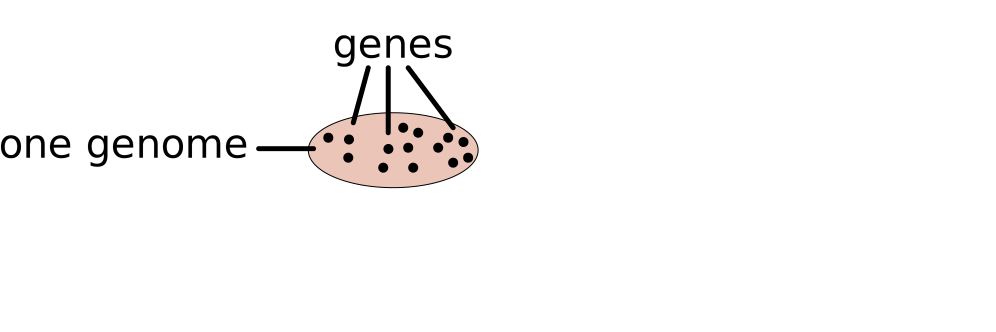
\includegraphics[width=\textwidth]{figs/pangenome-flower0}}%
\only<3>{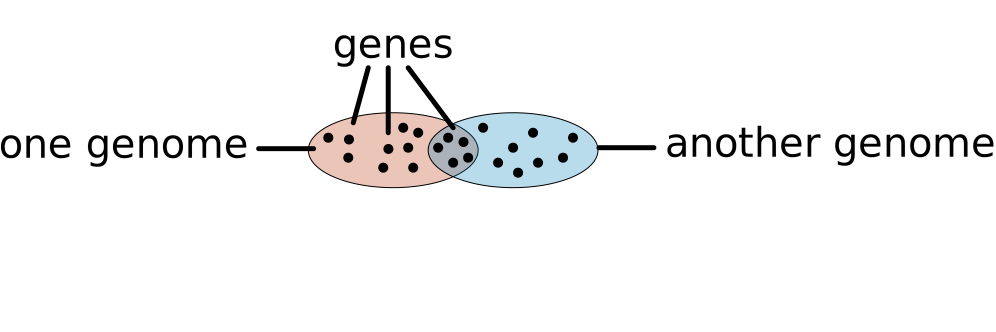
\includegraphics[width=\textwidth]{figs/pangenome-flower1}}%
\only<4>{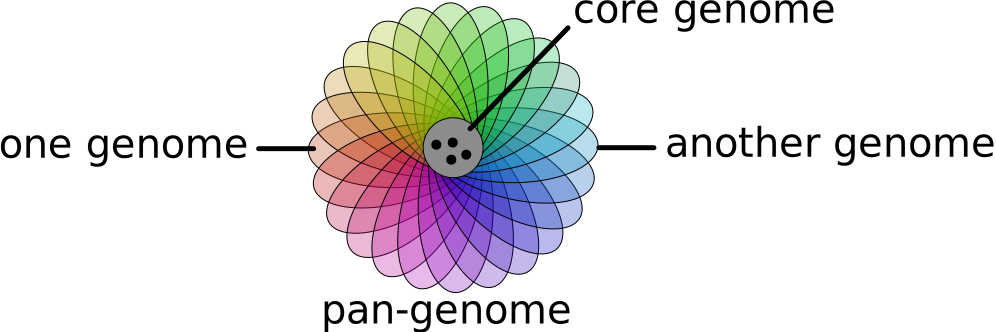
\includegraphics[width=\textwidth]{figs/pangenome-flower2}}%
\end{center}
}
\end{frame}

\begin{frame}[label=bacteria]
\frametitle{Pan-Genomes arise through Horizontal Gene Transfer (HGT)}
\begin{center}
\includegraphics[width=.5\textwidth]{figs/hgt_present}
\end{center}
\end{frame}

\begin{frame}{Mechanisms of Horizontal Gene Transfer}
\begin{columns}
\begin{column}{.55\textwidth}
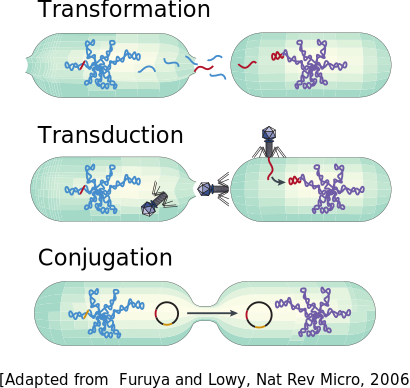
\includegraphics[width=\columnwidth]{figs/hgt-mechanisms}
\end{column}
\begin{column}{.45\textwidth}
\begin{block}{Relevance of HGT}
\begin{itemize}
 \item Outbreaks involving HGT (e.g.\ EHEC outbreak in Germany 2011)
 \item Transgenic and genetically modified organisms
 \item Antibiotic resistance can be acquired via HGT
\end{itemize} 
\end{block}
\end{column}
\end{columns}
\end{frame}

% \begin{frame}{Detecting Horizontal Gene Transfer}
% \begin{center}
% 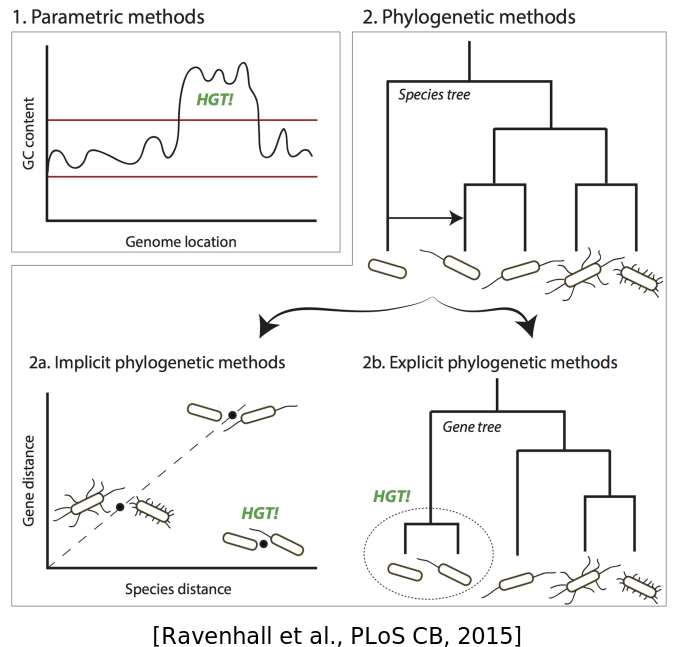
\includegraphics[height=.9\textheight]{figs/hgt-detection-paradigms}
% \end{center}
% \end{frame}
% 

\begin{frame}{Resistant Bacteria are Problem}
\begin{center}
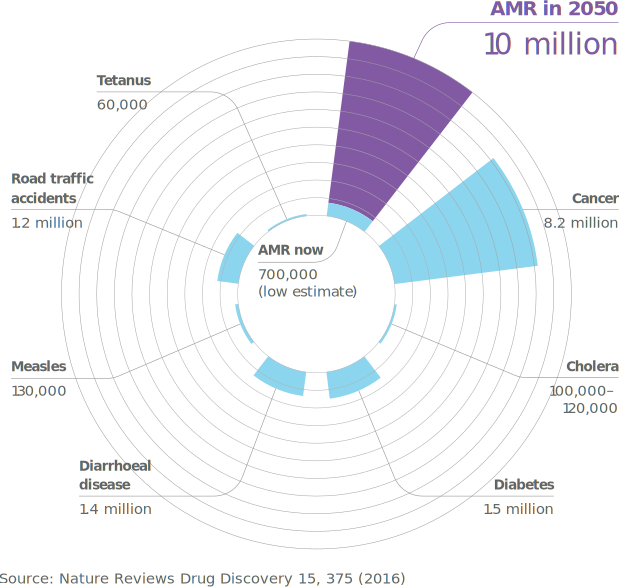
\includegraphics[width=.8\textwidth]{figs/amr-deaths}
\end{center}
\end{frame}

\begin{frame}{Mechanisms of Resistance}
\begin{center}
\only<1>{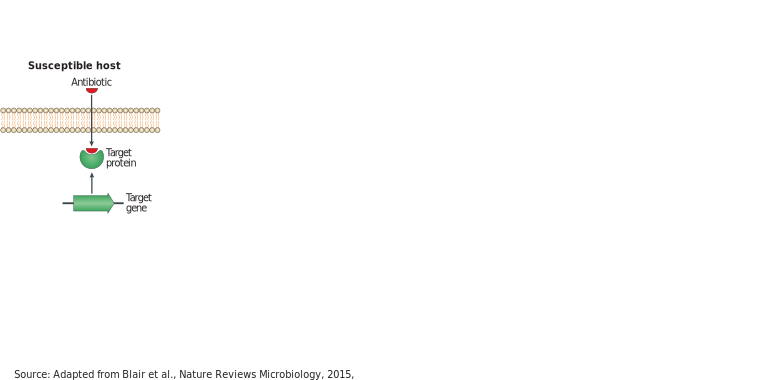
\includegraphics[width=\textwidth]{figs/resistance-mechanisms0}}%
\only<2>{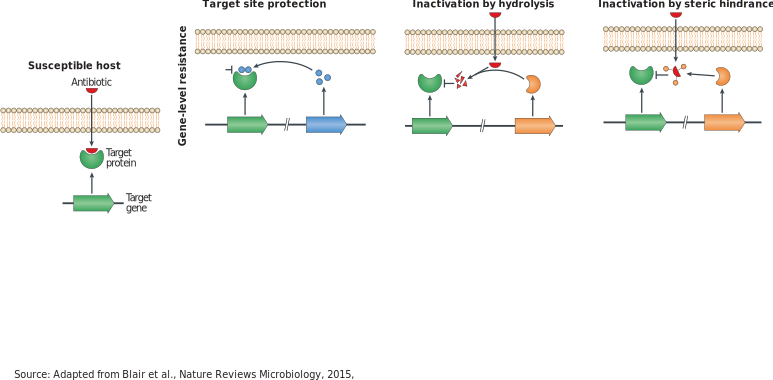
\includegraphics[width=\textwidth]{figs/resistance-mechanisms1}}%
\end{center}
\end{frame}

\begin{frame}{From Gene-Based to Sequence-Based Pan-Genomes}
\begin{block}{Question}
Are \emph{genes} really just \emph{absent or present}?
\begin{center}

\includegraphics[width=.45\textwidth]{figs/pangenome-flower1-notext}
\end{center}
\end{block}
\begin{block}<2->{Answer}
\only<1-4>{\emph{No}. Genes are encoded as \emph{sequences}.}
\uncover<3->{
\begin{center}
\only<1-3>{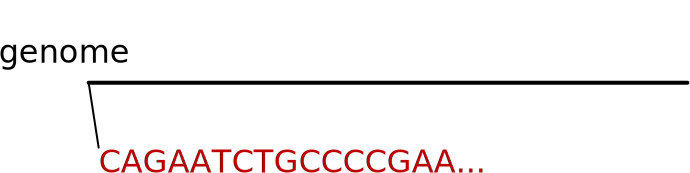
\includegraphics[width=.7\textwidth]{figs/genes-as-sequences1}}%
\only<4>{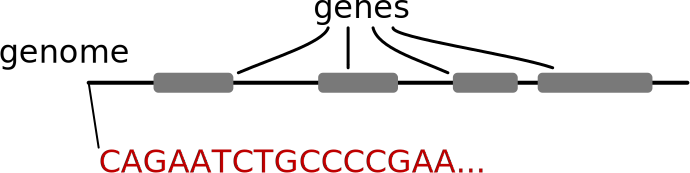
\includegraphics[width=.7\textwidth]{figs/genes-as-sequences2}}%
\only<5>{\includegraphics[width=.8\textwidth]{figs/genes-as-sequences-two-strains2}}%
\only<6>{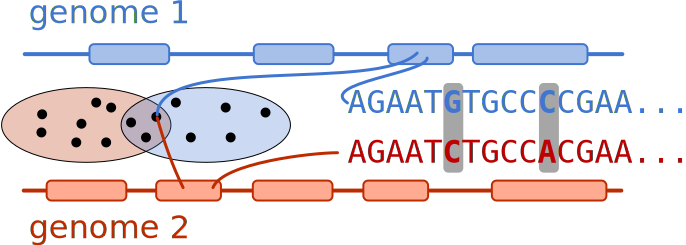
\includegraphics[width=.8\textwidth]{figs/genes-as-sequences-two-strains3}}%
% \only<7>{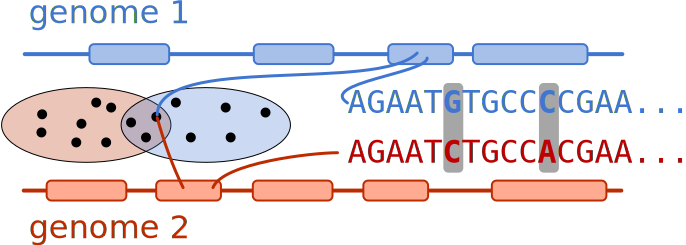
\includegraphics[width=.8\textwidth]{figs/genes-as-sequences-two-strains3}}%
\end{center}
}
\end{block}
\end{frame}


\begin{frame}{Mechanisms of Resistance}
\begin{center}
\only<1>{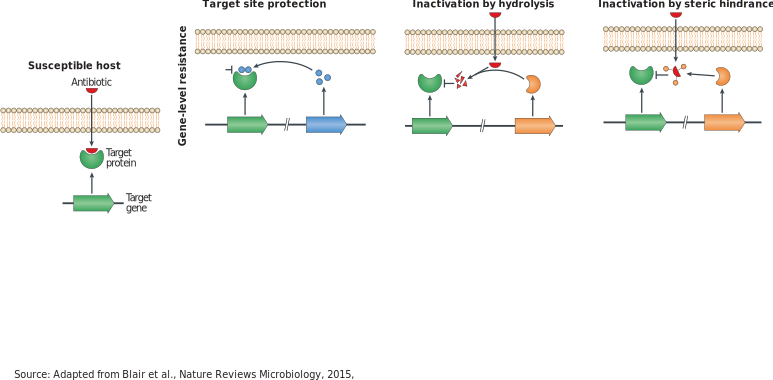
\includegraphics[width=\textwidth]{figs/resistance-mechanisms1}}%
\only<2>{\includegraphics[width=\textwidth]{figs/resistance-mechanisms2}}%
\end{center}
\end{frame}

\begin{frame}{Building a Bacterial Pan-Genome}
\begin{center}
\only<1>{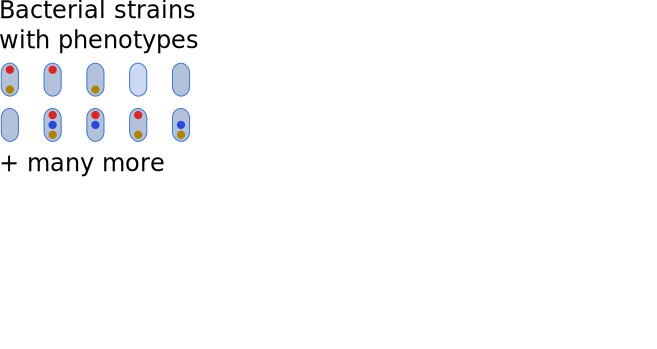
\includegraphics[width=\textwidth]{figs/building-bacterial-pangenome1}} %
\only<2>{\includegraphics[width=\textwidth]{figs/building-bacterial-pangenome2}} %
\only<3>{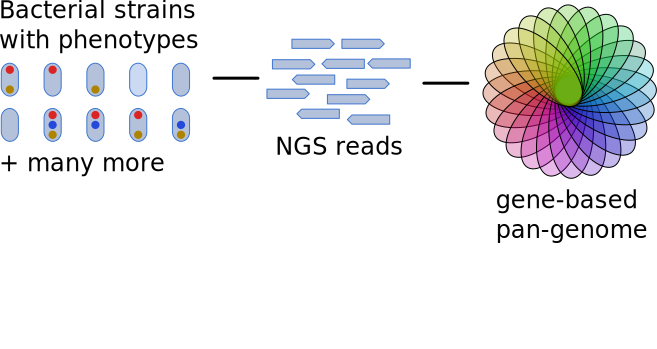
\includegraphics[width=\textwidth]{figs/building-bacterial-pangenome3}} %
\only<4>{\includegraphics[width=\textwidth]{figs/building-bacterial-pangenome4}} %
\only<5>{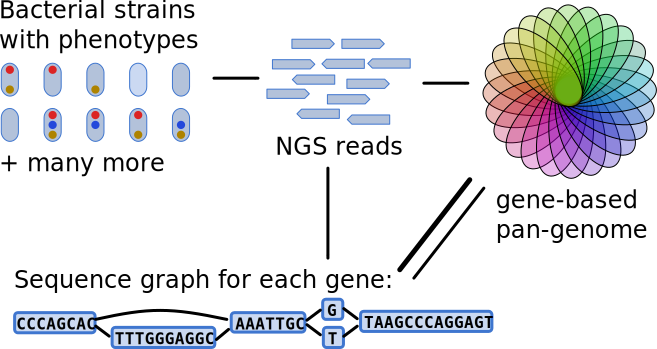
\includegraphics[width=\textwidth]{figs/building-bacterial-pangenome5}} %
\end{center}
\end{frame}


\begin{frame}{Towards Bacterial (Pan-)Genome-Wide Association Studies}
\begin{center}
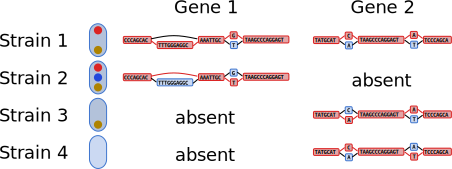
\includegraphics[width=\textwidth]{figs/bacterial-pangenome-gwas}
\end{center}
\end{frame}

\end{document}


